\documentclass{article}

\begin{document}
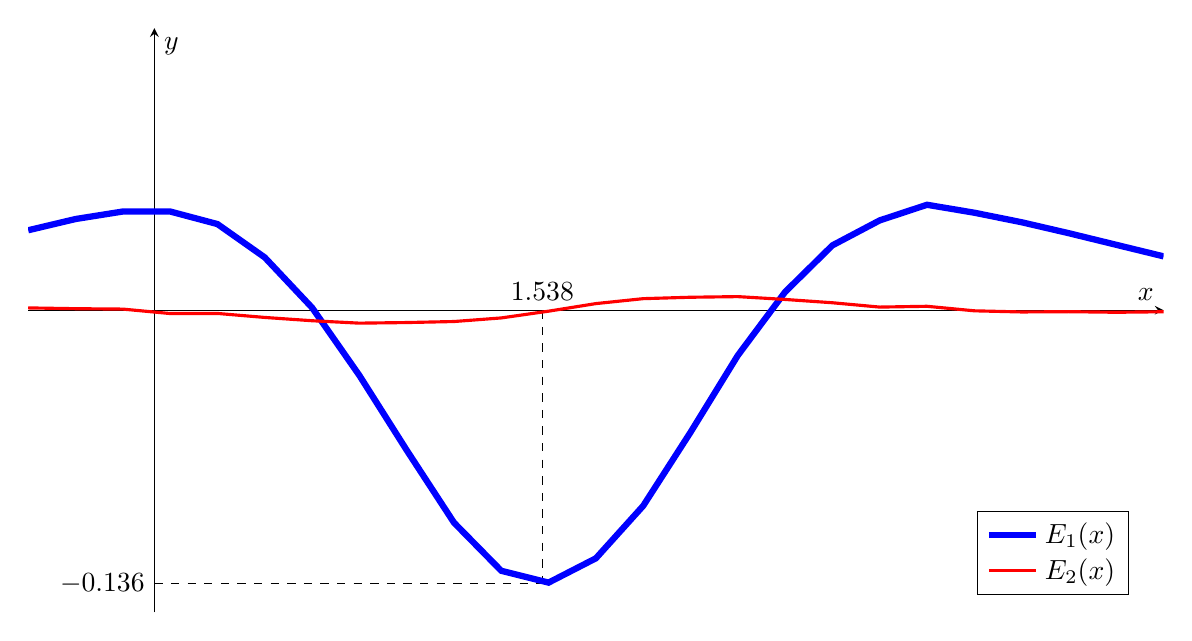
\begin{tikzpicture} [
	declare function= {
		toDeg(\r) = \r * 180 / pi;
		f(\x) = e^(sin (toDeg(\x)));
		der(\x) = cos (toDeg(\x)) * e^(sin(toDeg(\x)));
		app1(\x,\h) = (f(\x + \h) - f(\x)) / \h;
		app2(\x,\h) = (f(\x + \h) - f(\x - \h)) / 2 / \h;
	},]
	\begin{axis} [
		height=9cm,
		width=16cm,
		xlabel = {$x$},
		ylabel = {$y$},
		axis x line = middle,
		axis y line = middle,
		ymin = -0.15,
		ymax = 0.14,
		domain = -0.5:4,
		ticks = none,
		legend pos = south east]

		\newcommand*{\Shift}{0.1}
		\newcommand*{\Ax}{1.538}
		\pgfmathsetmacro{\Ay}{app1(\Ax,\Shift)-der(\Ax)}

		\pgfkeys{/pgf/number format/.cd,fixed,precision=3}
		\coordinate(A) at	(\Ax,\Ay);
		\node[above](Ax) at	(\Ax, 0) {\Ax};
		\node[left](Ay) at	(0, \Ay) {\pgfmathprintnumber{\Ay}};

		\draw[dashed] (Ax) -- (A) (Ay) -- (A);

		\addplot[color=blue,line width=0.8mm] {app1(x,\Shift)-der(x)};
		\addplot[color=red,line width=0.4mm] {app2(x,\Shift)-der(x)};

		\addlegendentry{$E_1(x)$};
		\addlegendentry{$E_2(x)$};
	\end{axis}
\end{tikzpicture}
\end{document}
